\begin{figure}[H]
        \centering
        \label{fig:block}
        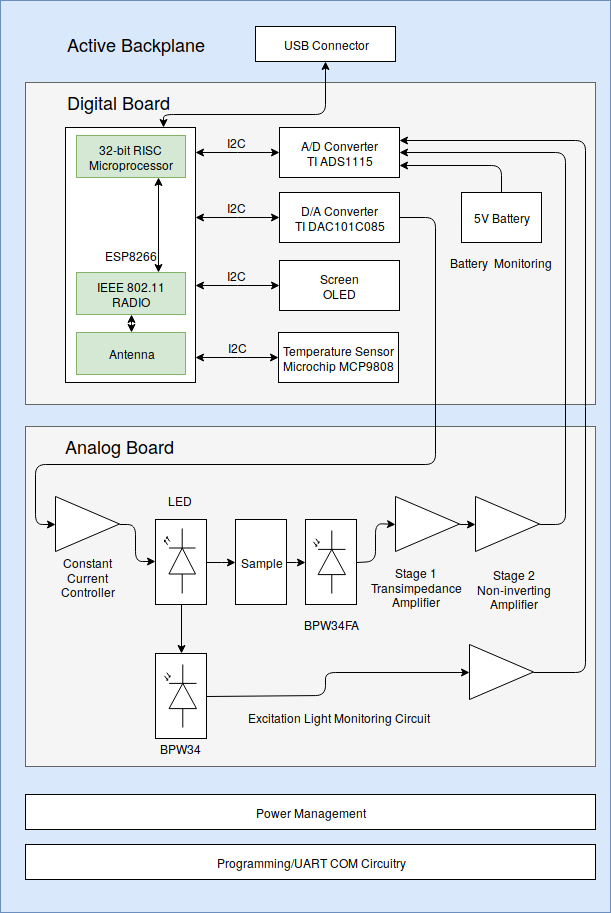
\includegraphics[width=0.6\textwidth]{../block/block.png}
        \caption{Blockdiagram of the Swakeup wakeup light.}
\end{figure}
In fig. \ref{fig:block} the actual system architecture from an abstract point of view is displayed. One can clearly see, that the system is divided into two physical boards. The logic board consists of the µC, a serial connection infrastructure, an OLED screen, an \textit{IEEE 802.11} module, a ISP programming infrastructure and some LEDs/a button (UI).
\newpar  
The power board takes the 20 V input of a low-cost power supply and breaks it down to 2.8 V (Vcc), 5 V for phone charging and the power which is needed for the RGB LED.
\newpar
The partitioning of the system functionalities on two boards has a bunch of advatages: Two people worked on this project, so each could develop a PCB; It is quite common to seperate signals from power lines out of EMI reasons; There was simply not eanough space on one two-layer board for the whole system keeping a base area of 5 cm x 4 cm. 
\newpar
The two boards are connected together through four headers. By these headers an electrical and mechanical connection is maintained. The headers allow a feedback from the LED driver on the power board to the logic board (ADC). Also the control variable (PWM) comes via the headers from the µC to the LED driver. The 2.8 V Vcc is produced and regulated on the power board and is also availabe at one header. Another voltage available from one header is the OLED driver voltage.       
